% Created 2018-04-30 Mon 05:24
\documentclass{article}
\usepackage[mathletters]{ucs}
\usepackage[utf8x]{inputenc}
\usepackage[T1]{fontenc}
\usepackage{fixltx2e}
\usepackage{graphicx}
\usepackage{longtable}
\usepackage{float}
\usepackage{wrapfig}
\usepackage{rotating}
\usepackage[normalem]{ulem}
\usepackage{amsmath}
\usepackage{textcomp}
\usepackage{marvosym}
\usepackage{wasysym}
\usepackage{amssymb}
\usepackage{hyperref}
\tolerance=1000
\date{\today}
\title{notebook}
\hypersetup{
  pdfkeywords={},
  pdfsubject={},
  pdfcreator={Emacs 25.3.1 (Org mode 8.2.10)}}
\begin{document}

\maketitle
\tableofcontents

\section{Information}
\label{sec-1}
\begin{itemize}
\item So this pdf will basically follow the matlab notebook and each section
will be linked to the corresponding section in the matlab notebook.
\item This will just commentate on the code given, not add any extra code
\item This is being done as I can easily manipulate an org file as
it's not too difficult to mess with formatting
\item Throughout this file I'll probably explain a lot about the matlab
code since it's foreign.
\end{itemize}
\section{Build a simple Virtual world}
\label{sec-2}
\begin{enumerate}
\item Add something into the world
\label{sec-2-1}
\begin{itemize}
\item so this creates a function called
\texttt{create\_points()}. \texttt{create\_points()} starts off by creating a 3dmesh
grid with values -5,0,5
\begin{itemize}
\item A mesh grid in this case seems create a 3d array for X, Y, and Z
such that the shift of values for the values for X shifts along
the X axis (so \texttt{X(1,:,:)} has all the variations), the values for
Y shifts along the Y axis (so \texttt{Y(:,1,:)} has all the variation), and
the value for the Z axis changes on the Z axis (so \texttt{Z(:,:,1)} has
all the variation)
\end{itemize}
\item The last thing is that we get the jet of the length of points (which
is just 3$^{\text{3}}$ = 27)
\begin{itemize}
\item Jet returns some kind of color-map with the specified length
\end{itemize}
\item Nothing too interesting happening here
\end{itemize}
\item Plot the points
\label{sec-2-2}
\begin{itemize}
\item So the code in the above section generates this graph here
\item 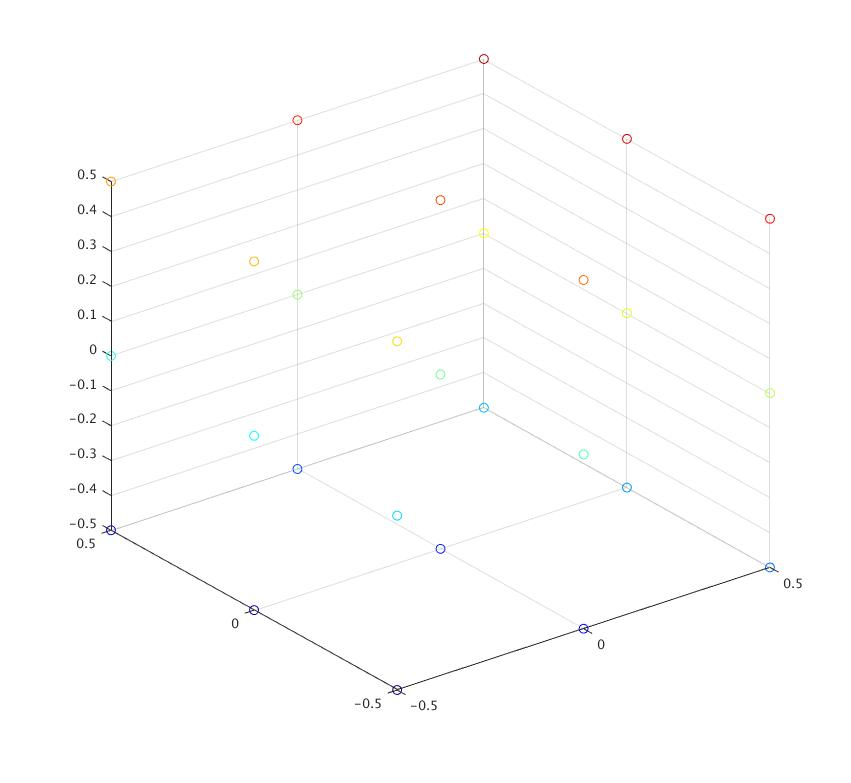
\includegraphics[width=.9\linewidth]{plot-the-points.jpg}
\item which we can see is just a 3x3 grid with the colors given by the
color map
\item The code itself just explains a scatter plot of the X Y and Z
variables defined above with the colors applied
\end{itemize}
\item Set up a pair of Cameras
\label{sec-2-3}
\begin{itemize}
\item So this code sets up 2 cameras, both with the exact same function
just not abstracted out. The only difference is the α variable given
\item this beta only shows up in the position of the camera, and the 3rd
position does not rely on α at all so it can only effect the first two
values of the array.
\item We can also notice that $\sin(\frac{π}{3})$ = $\cos(\frac{π}{6})$
which means that the only difference between the cameras is that the
first two positions of the camera are swapped, since the only
difference is that one is cos(alpha) vs sin(alpha) (which swap with
each other when π/6 turns into π/3)
\item Therefor the could be improved in this particular instance by
instead writing
\item Other values on the camera struct are the following
\begin{itemize}
\item \uline{up}
\begin{itemize}
\item This is the vector for the camera up direction
\end{itemize}
\item \uline{Target}
\begin{itemize}
\item This is the point in which the camera is looking (which in this
case is [0 0 0] which is the origin)
\end{itemize}
\item \uline{\texttt{focal\_length}}
\begin{itemize}
\item this is how far out the rectangle the camera projects is
\end{itemize}
\item \uline{\texttt{film\_width}}
\begin{itemize}
\item this will be used to get the width of the rectangle of the
rectangle that the camera projects with respect to the focal length
\end{itemize}
\item \uline{\texttt{film\_height}}
\begin{itemize}
\item Like width but for height
\end{itemize}
\end{itemize}
\begin{verbatim}
for fn = fieldnames(cam2)'
cam2.(fn{1}) = cam1.(fn{1});
end
cam2.position([1 2]) = cam2.position([2 1])
\end{verbatim}
\begin{itemize}
\item of course a more generic function that took β and α would be better
and allow for more kinds of behavior
\end{itemize}
\end{itemize}
\item Plot camera
\label{sec-2-4}
\begin{itemize}
\item the \texttt{camera\_coordinate\_system} is rather interesting here because we
can note for the two cameras we are using zcam is really just (-
cam.position) since both cameras have a [0 0 0] for target, which
means. The rest of the function does math that is already commented
in the file.
\item The next section after this just goes through with details of
trying to get the rectangle that camera sees
\item it uses details like \texttt{film\_width} and \texttt{film\_length} to determine the
corners of the rectangle the camera projects as it looks towards
it's target (in this case the origin)
\end{itemize}
\end{enumerate}
\section{Show the virtual world}
\label{sec-3}
\begin{itemize}
\item The first section shows the output values of the camera, which the
differences were already discussed in \hyperref[sec-2-3]{Set up a pair of Cameras}
\item The second and third section just plot the camera and show the side by
side of where they are located
\end{itemize}
\section{Camera Model}
\label{sec-4}
\begin{enumerate}
\item Euclidean Transformation matrix
\label{sec-4-1}
\begin{itemize}
\item So this transformation deals with the reflection when light hits a
surface at an angle
\item in the case of the code this surface can be seen as the origin, and
the vector given back could be seen as r$_{\text{1}}$' on the slides, which we
can tell since the code returns [R; -origin*R] where R = [xcam(:),
ycam(:), zcam(:)], which we can visualize the change as the
following from camera1
\begin{verbatim}
>> [xcam;ycam;zcam;origin]

ans =

   -0.5000    0.8660         0
    0.4330    0.2500   -0.8660
   -0.7500   -0.4330   -0.5000
    3.7500    2.1651    2.5000

>> ExtrinsicsMtx(cam1)

ans =

   -0.5000    0.4330   -0.7500
    0.8660    0.2500   -0.4330
         0   -0.8660   -0.5000
   -0.0000         0    5.0000
\end{verbatim}
\begin{itemize}
\item if we ignore the bottom rows of both matrices, we are just doing a
diagonal flip down the center of the matrix, essentially
achieving the change from r$_{\text{1}}$ to r$_{\text{1}}$' in the image below
\begin{itemize}
\item 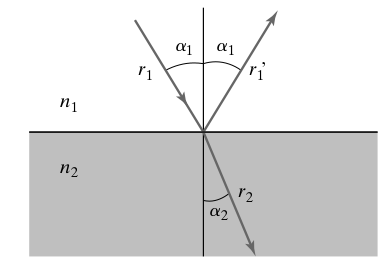
\includegraphics[width=.9\linewidth]{reflected.png}
\end{itemize}

\item As for the bottom row of each matrix, we can see that origin is
the starting location of camera1, and the new location is what I'm
guessing is the image is being projected from [0 0 5] which can be
seen as the new origin of the camera instead of the original origin.
\end{itemize}
\end{itemize}
\item Camera Calibration matrix
\label{sec-4-2}
\begin{itemize}
\item 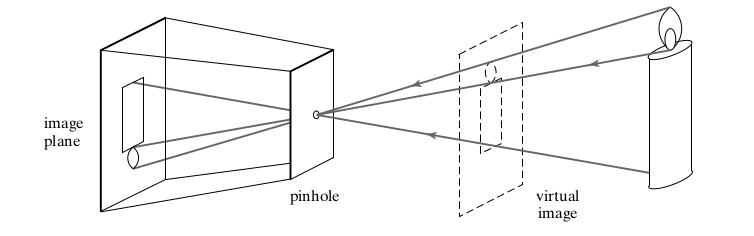
\includegraphics[width=.9\linewidth]{light.png}
\item The slide on page 4 describes viewing an image through a pinhole and
seeing the inverse image.
\item In our case, the pinhole would be our camera lens, and the outlining
sketch of the candle (virtual image) would correspond to the
rectangle drawn previously that depends on the \texttt{focal\_length} and the
height and width.
\item Ι can't visualize exactly the transformation of the diagram to the
code here, but Ι do notice there is 4 0s in the returned matrix,
which I think has to do with wasting light which is described on
slide 5. it would make sense that some information would thus be
wasted with this model of the camera.
\end{itemize}
\item Camera Matrix
\label{sec-4-3}
\begin{itemize}
\item The previous two come together, and we should note the names of the
functions, one is extrinsic and the other is intrinsic, which we can
see in the way they view the world. the first one views it as a
reflection on the surface and the other views it as lights converging
on it, which seem to reflect the image on slide 7
\item 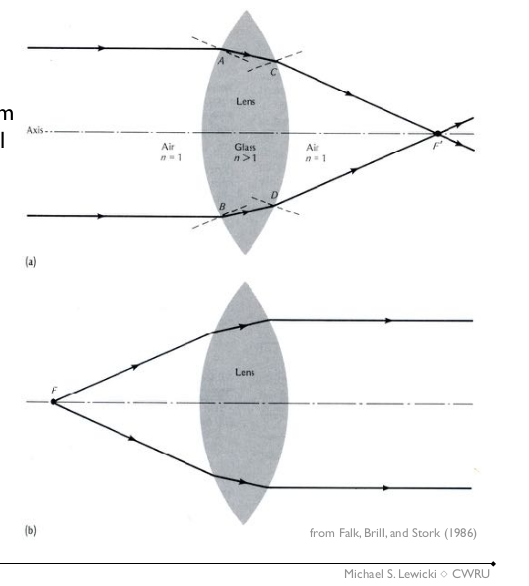
\includegraphics[width=.9\linewidth]{lens.png}
\end{itemize}
\item Generate the Image Pair
\label{sec-4-4}
\begin{itemize}
\item it seems here we do some math to construct the 2d projection of the
3d image, I'm not exactly sure of the math that is happening here that
dictates the placement of the points
\item the second section in this file is the set-Color function which does
some math to colorize each point differently
\item After this we just plot both cameras, and see that the structure looks
like our original structure from both images (scroll back up to look
through camera 2, and look through camera 1, you can tell they look
very similar) just at different angles from our
original two cameras.
\end{itemize}
\end{enumerate}
\section{Triangulation}
\label{sec-5}
\begin{itemize}
\item Since we have 2 2d projection we can try to recover the 3d
information
\item Really this can be done by solving a linear equation from the images
given for every point in common
\end{itemize}
\begin{enumerate}
\item Linear Triangulation method
\label{sec-5-1}
\begin{itemize}
\item \texttt{triangulationOnePoint} basically seems to solve the triangulation of
two points given to it from the corresponding images, though doing
some transformations with the 2 vectors gathered from the cameras in
the last section.
\item From here we just map this triangulation over all the shared points
between the two images
\item Note that nothing in this algorithm is really specialized for 2
images, one can generalize this to n-images by sending in 2 lists, 1
of the points and 1 of the 2d matrices of the camera, essentially just
doing this equation with more matrices.
\item Finally we plot the 3d structure and see that it isn't too different
from the original 3d image that is at the start of this document
\item The final section just adds some noise into the image, and as one can
see, the noise doesn't really hurt the representation of the
structure much, and it pretty much stays in tact
\end{itemize}
\end{enumerate}
% Emacs 25.3.1 (Org mode 8.2.10)
\end{document}